%\section{编译环境简介}
%在开发应用程序时,高级语言是必不可少的工具。利用高级语言开发自然离不开高级语言编译器,而GCC(GNU Compiler Collection)就是目前Linux下最常用的高级语言编译器。GCC是GNU推出的功能强大的编译器套件,是GNU项目中符合ANSI C标准的编译系统,能够编译使用C、C++、Objective-C等语言编写的程序;同时,GCC也可以在多种硬件平台上编译出可执行程序,且具有较高的执行效率。\\
%“工欲善其事,必先利其器”。本部分对GCC编译系统的相关内容予以介绍。
%
%\subsection{GCC编译器简介}
%GCC是以GPL许可证所发行的自由软件,也是GNU计划的关键部分。GCC的初衷是为GNU操作系统专门编写一款编译器,现已被大多数类Unix操作系统(如Linux、BSD、MacOS X等)采纳为标准的编译器,甚至在微软的Windows上也可以使用GCC。GCC支持多种计算机体系结构芯片,如x86、ARM、MIPS等,并已被移植到其他多种硬件平台。
%GCC原名为GNU C语言编译器(GNU C Compiler),只能处理C语言。但其很快扩展,变得可处理C++,后来又扩展为能够支持更多编程语言,如Fortran、Pascal、Objective -C、Java、Ada、Go以及各类处理器架构上的汇编语言等,所以改名GNU编译器套件(GNU Compiler Collection)。\\
%
%GCC允许程序员将编译过程中得到的语法中间表示导出为数据文件,程序员可以通过该中间文件直接获取 GCC 编译代码过程中的内部信息。本报告所要研究的是编译器在编译程序过程中的工作流程,因此通过制定编译选项来查看产生的中间文件,可以大大降低我们的分析难度。因此,在本次报告中,我们以Linux环境下GCC编译器编译factorial.cpp的过程作为分析样例,来探究\textbf {预处理器}、\textbf {编译器}、\textbf {汇编器}、\textbf {链接器}四个部分在程序编译过程中发挥的功能。
%
%
%%\subsection{gcc命令与g++命令的介绍与比较}
%
%%\subsubsection{gcc与g++简介}
%%前文已经介绍过,GCC是指GUN 编译器套件(GNU Compiler Collection),它可以编译C、C++、JAVA、Fortran、Pascal、Object-C、Ada等多种语言。\\
%%
%%而gcc是GCC套件中的C编译器,即GUN C Compiler;g++则是GCC套件中的C++编译器,即GUN C++ Compiler。\\
%%
%%更深一步来讲,gcc和g++本质上并不是编译器,更不是编译器集合,而只是一种驱动器。根据参数中要编译的文件的类型,gcc和g++会调用对应的GUN编译器进行编译。所以,更准确的说法是:gcc调用了C Compiler,而g++调用了C++ Compiler\\
%%
%%既然gcc和g++只负责调用编译器的驱动器,而不是直接编译C和C++程序的编译器,那么也就不难理解这样一个事实:gcc和g++都是可以处理C语言源程序和C++语言源程序的。
%%
%%
%%其实,g++处理程序时,在编译阶段,g++驱动器会调用gcc驱动器,由gcc按照处理C++程序的方式进行处理,即编译工作最终都是由gcc来完成的;而链接阶段的工作则由g++自己来完成,因为gcc命令不能自动和c++程序使用的库连接,而g++才能自动调用链接的c++库。这一特性也导致两者在处理源程序时是有所区别的。下文对两者的主要区别进行阐释。
%%
%%\subsubsection{gcc命令与g++命令比较}
%%gcc和g++的主要区别有以下几点:
%%
%%\begin{itemize}
%%	\item gcc把.c后缀的文件\textbf{当做是C程序},把.cpp后缀的文件\textbf{当做是C++程序};g++把.c后缀和.cpp后缀的文件\textbf{都统一当做是C++程序}。
%%	
%%	\item 使用g++处理文件时,g++\textbf{会自动链接标准库STL};使用gcc处理文件时,gcc则\textbf{不会自动链接标准库STL}。因此,使用gcc处理c++文件时,为了能够使用STL,需要加参数 "–lstdc++"来手动链接C++库,指令形如"gcc factorial.cpp -lstdc++"。
%%	
%%	\item gcc在处理.c后缀文件时,可使用的预定义宏是比较少的;gcc在处理.cpp后缀文件以及g++在处理.c后缀文件和.cpp后缀文件时,会加入一些额外的宏。涉及gcc与g++差异的有关宏的定义参见附录1。	
%%\end{itemize}
%
%
%\subsection{GCC编译器基本用法}
%
%使用gcc指令编译程序的基本指令格式是:
%\begin{verbatim}
%      gcc  [options] filenames
%\end{verbatim}
%
%其中的参数含义如下:
%\begin{verbatim}
%      options :编译器所需要的编译选项,为可选参数,可以没有
%      filenames :要编译的文件名
%\end{verbatim}
%
%同时,通过设置编译选项,我们可以获得GCC编译器在编译过程中生成的中间文件。下面以编译factorial.cpp源程序为例,展示相应使用到的基本gcc指令。
%
%%\begin{figure}[thbp!]
%%	\centering
%%	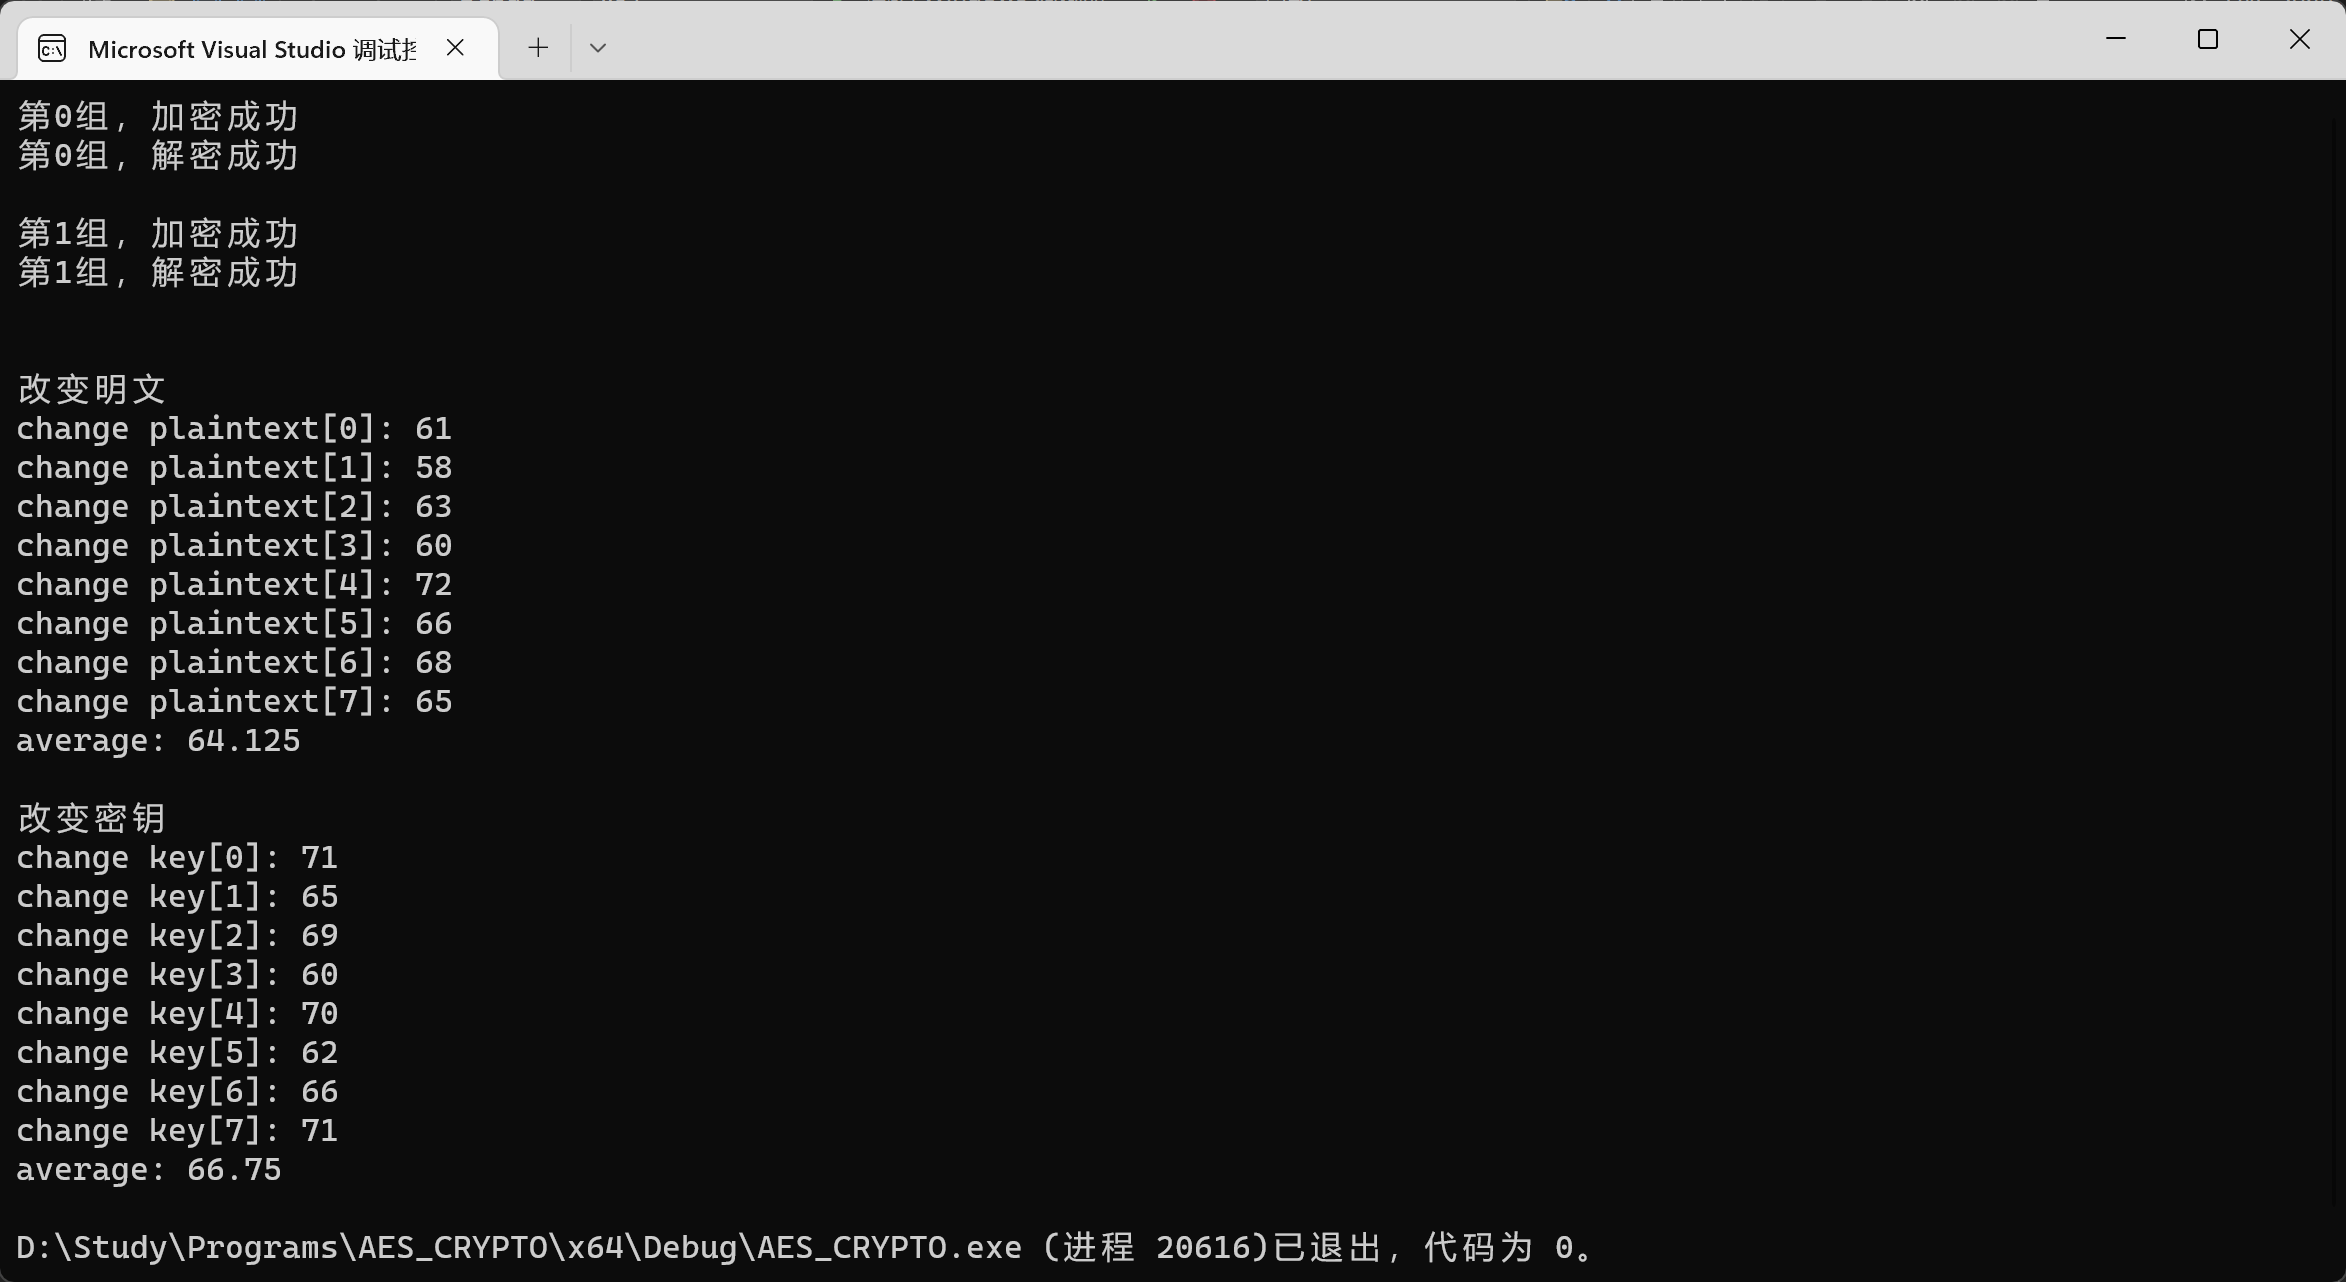
\includegraphics[height=6.8 CM]{figure/002}
%%	\caption{gcc基本指令示意}
%%	\label{fig:gcc基本指令示意}
%%\end{figure}
%
%%\begin{figure}[thbp!]
%%	\centering
%%	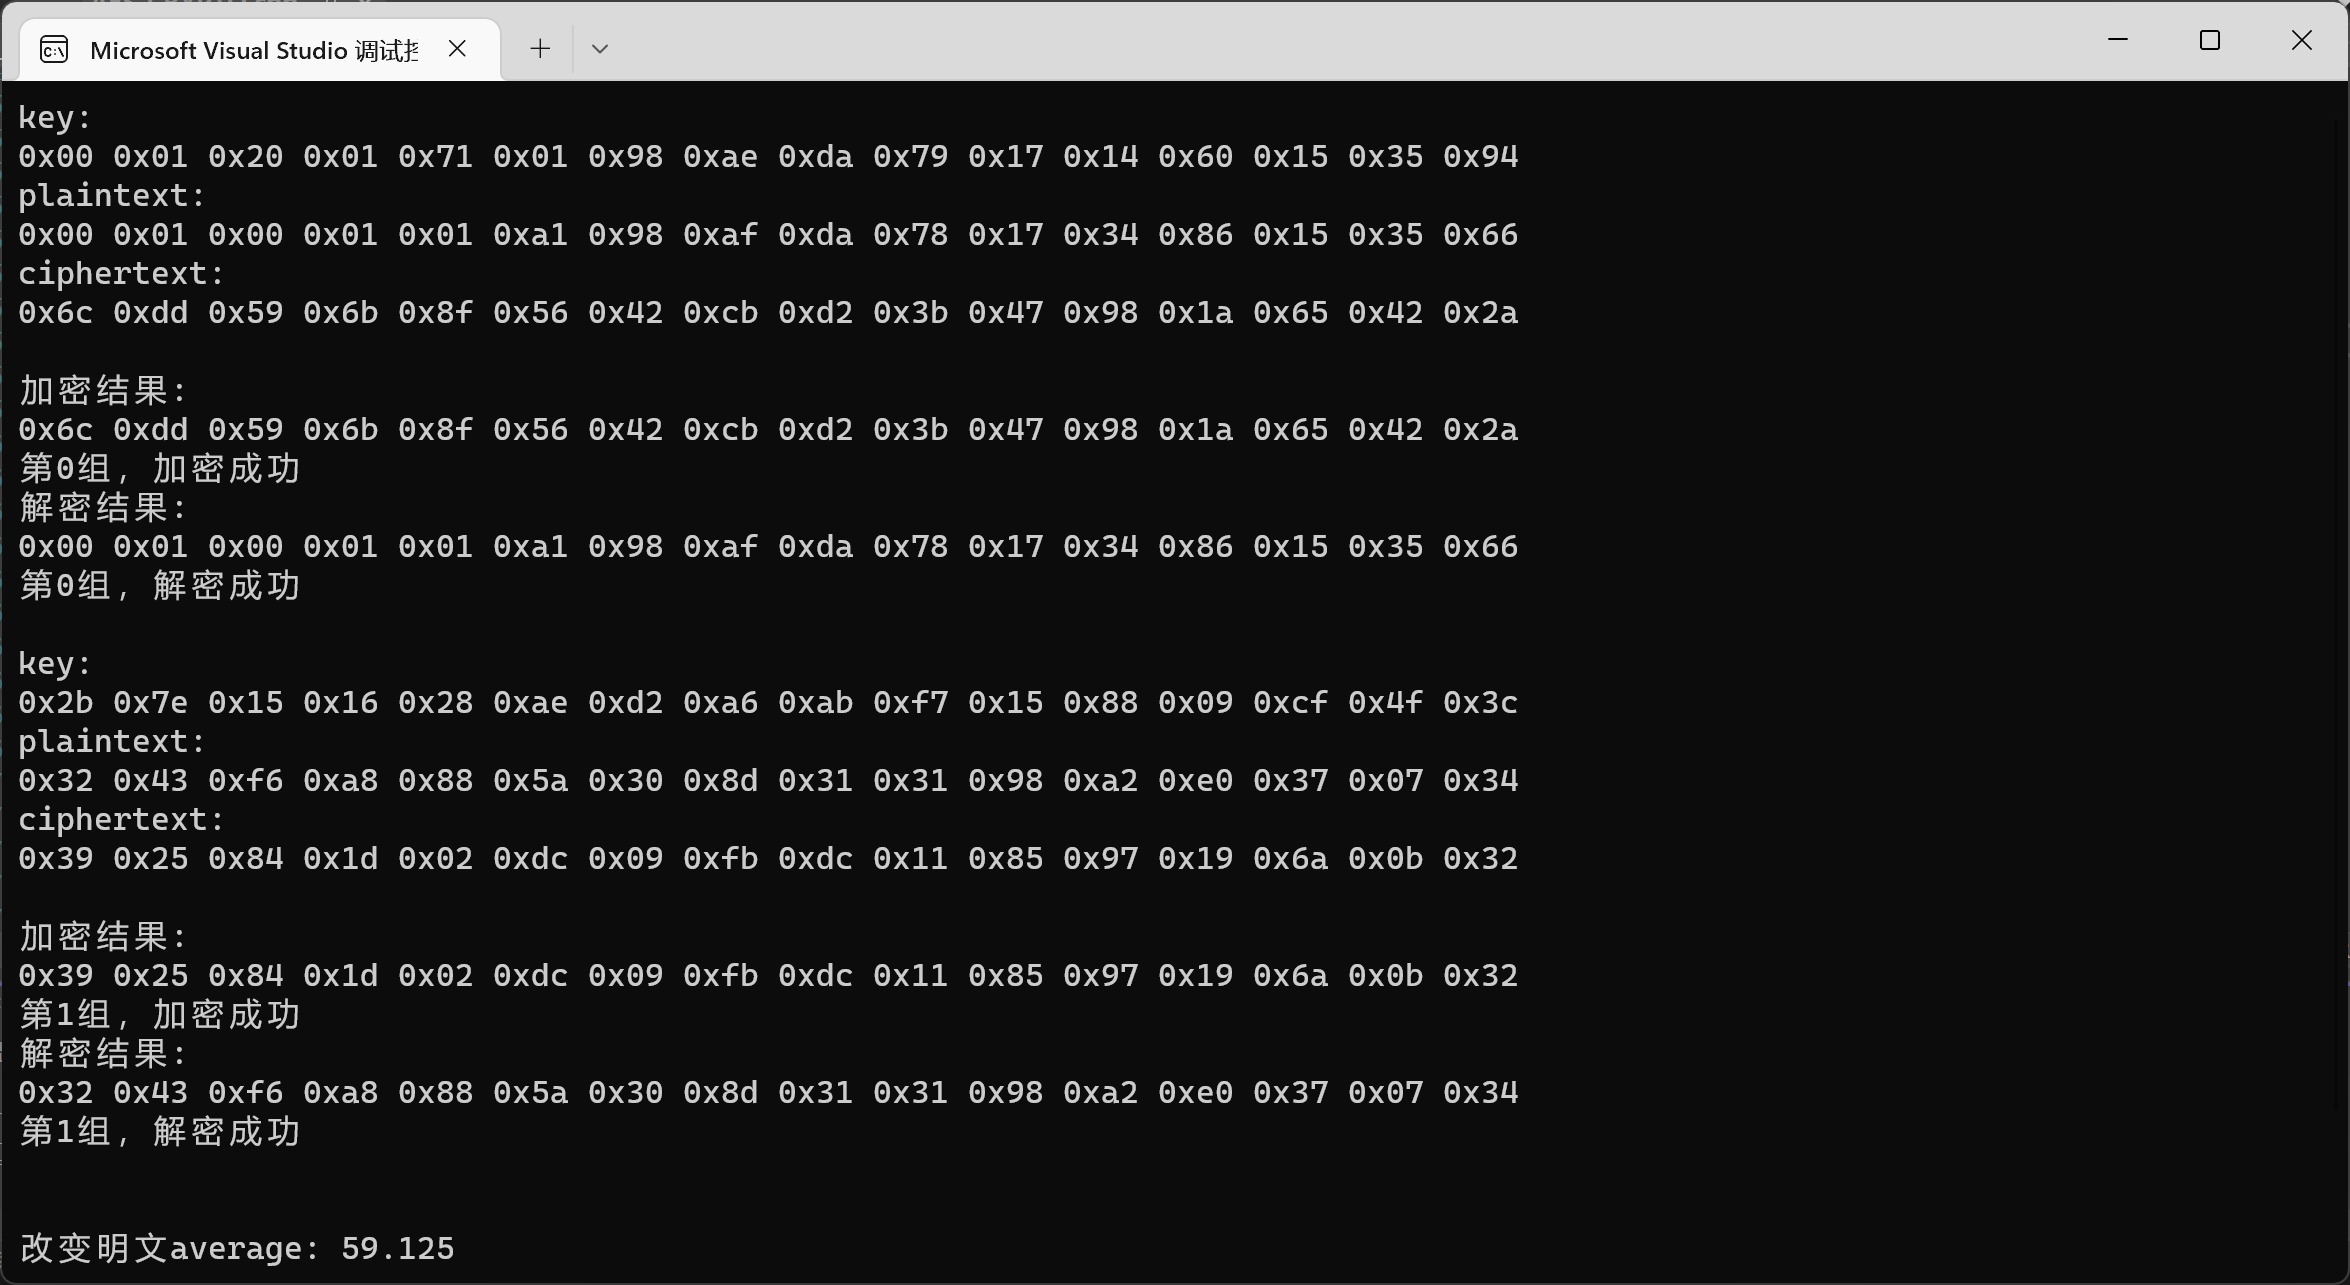
\includegraphics[height=10 CM]{figure/003}
%%	\caption{gcc中间结果文件关系示意}
%%	\label{fig:gcc中间结果文件关系示意}
%%\end{figure}
%
%%\subsection{实验环境信息}
%%本报告中,我们以用C++语言编写的阶乘源程序factorial.cpp为例,分析其经过预处理得到的中间文件factorial.i。其中,所使用的Linux发行版操作系统版本为Ubuntu 16.04.5,所使用的GCC编译器版本为GCC 5.4.0 20160609,如下图所示:\\
%%
%%\begin{figure}[thbp!]
%%	\centering
%%	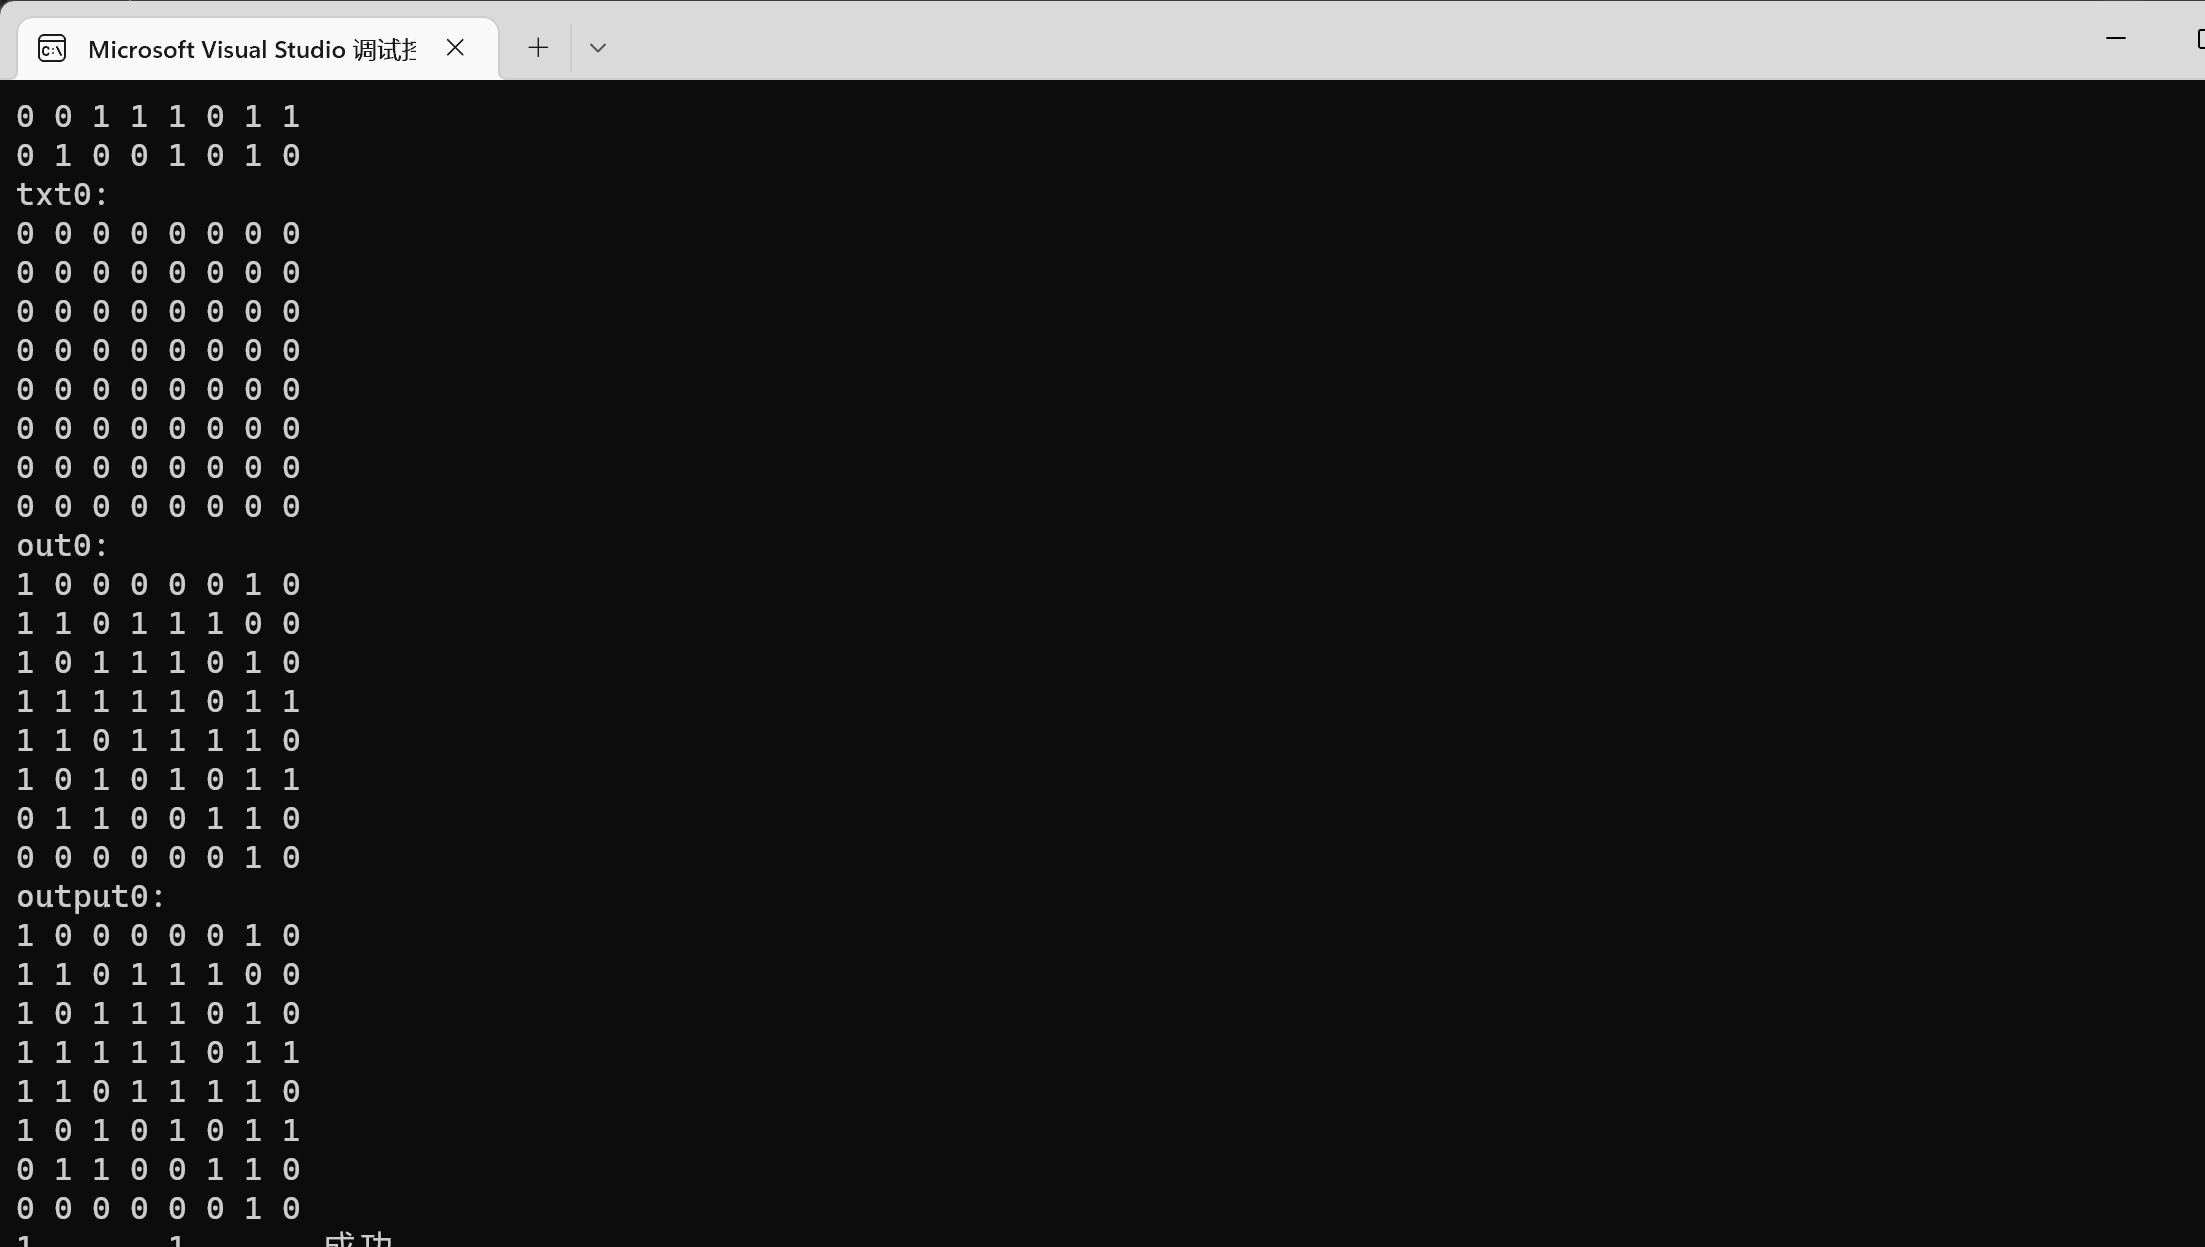
\includegraphics[height=7 CM,width=16 CM]{figure/004}
%%	\caption{操作系统及编译器版本}
%%	\label{fig:操作系统及编译器版本}
%%\end{figure}
%%
%%需要说明的是,本实验中使用的例程为C++语言编写的程序。为了能得到完整的包括C++库链接在内的编译过程,本次实验使用了g++指令。如前文所述,g++与gcc均属于GCC的驱动器,所以两者对应的编译器版本是完全相同的,均为GCC 5.4.0 20160609,如下图所示:
%%
%%\begin{figure}[htbp!]
%%	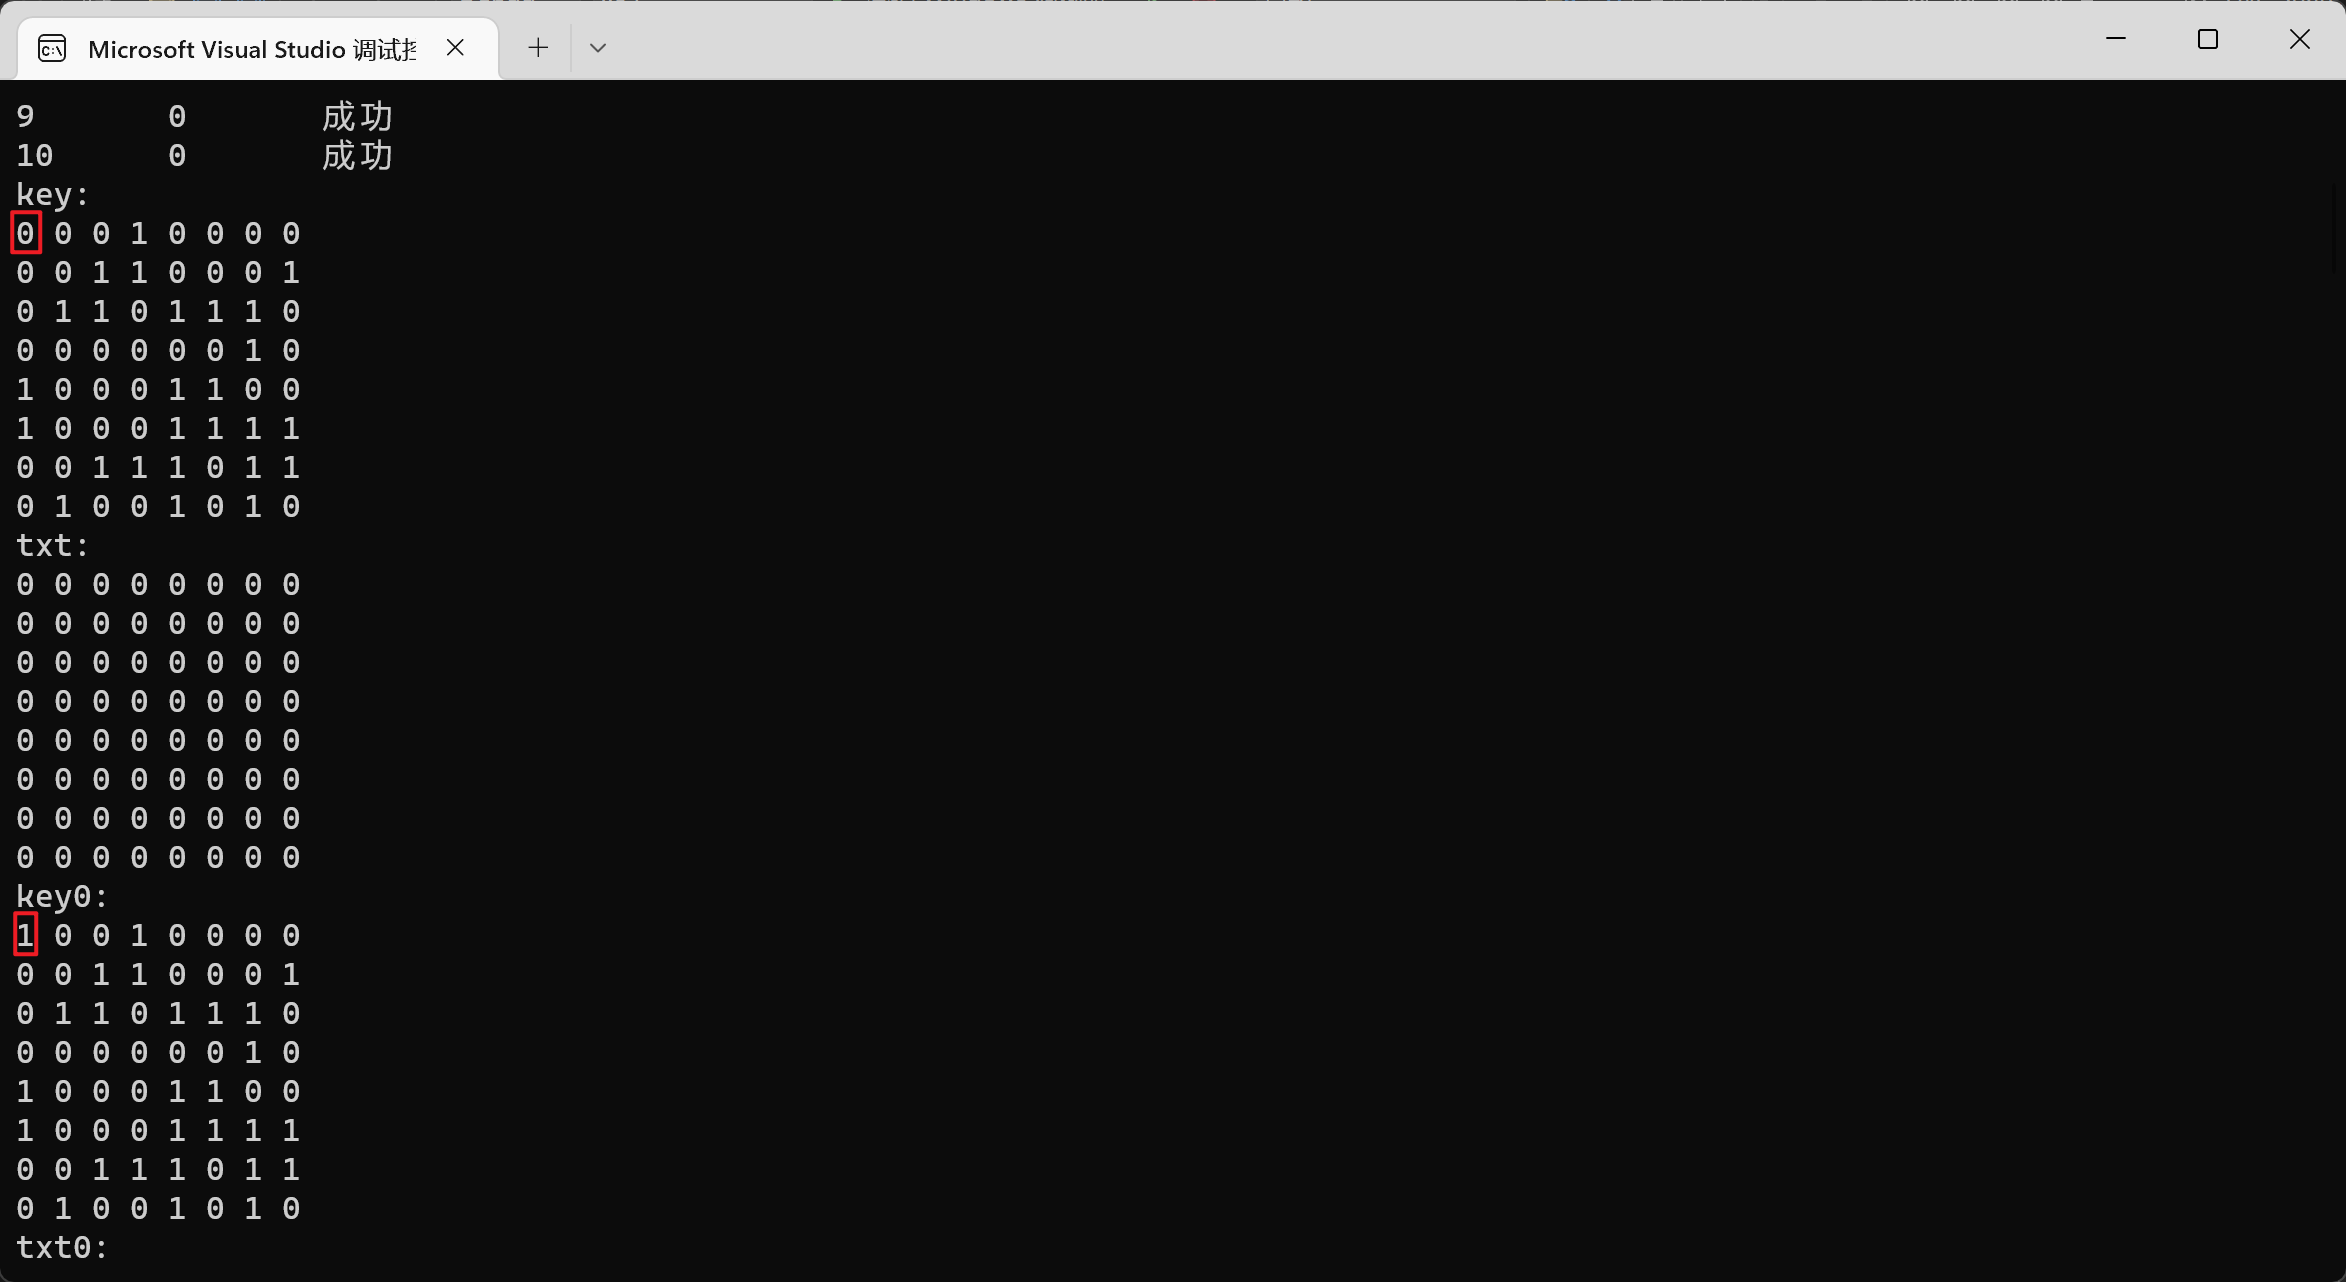
\includegraphics[height=7 CM,width=16 CM]{figure/005}
%%	\caption{gcc与g++指令对应编译器版本信息比较}
%%	\label{fig:gcc与g++指令对应编译器版本信息比较}
%%\end{figure}
%
%
%
%
%
%
%
%
%
%
%
%
%
%
%
%
%
%
%
%
%
%
%
